%% Copernicus Publications Manuscript Preparation Template for LaTeX Submissions
%% ---------------------------------
%% This template should be used for copernicus.cls
%% The class file and some style files are bundled in the Copernicus Latex Package which can be downloaded from the different journal webpages.
%% For further assistance please contact the Copernicus Publications at: publications@copernicus.org
%% http://publications.copernicus.org


%% Please use the following documentclass and Journal Abbreviations for Discussion Papers and Final Revised Papers.


%% 2-Column Papers and Discussion Papers
\documentclass[gmd, manuscript]{copernicus}



%% Journal Abbreviations (Please use the same)

% Atmospheric Chemistry and Physics (acp)
% Advances in Geosciences (adgeo)
% Advances in Statistical Climatology, Meteorology and Oceanography (ascmo)
% Annales Geophysicae (angeo)
% ASTRA Proceedings (ap)
% Atmospheric Measurement Techniques (amt)
% Advances in Radio Science (ars)
% Advances in Science and Research (asr)
% Biogeosciences (bg)
% Climate of the Past (cp)
% Drinking Water Engineering and Science (dwes)
% Earth System Dynamics (esd)
% Earth Surface Dynamics (esurf)
% Earth System Science Data (essd)
% Fossil Record (fr)
% Geographica Helvetica (gh)
% Geoscientific Instrumentation, Methods and Data Systems (gi)
% Geoscientific Model Development (gmd)
% Geothermal Energy Science (gtes)
% Hydrology and Earth System Sciences (hess)
% History of Geo- and Space Sciences (hgss)
% Journal of Sensors and Sensor Systems (jsss)
% Mechanical Sciences (ms)
% Natural Hazards and Earth System Sciences (nhess)
% Nonlinear Processes in Geophysics (npg)
% Ocean Science (os)
% Primate Biology (pb)
% Scientific Drilling (sd)
% SOIL (soil)
% Solid Earth (se)
% The Cryosphere (tc)
% Web Ecology (we)


\begin{document}

\linenumbers

\title{An automatic and effective parameter optimization method for model tuning}


% % \Author[affil]{given_name}{surname}

\Author[1]{Tao}{Zhang}
%\Author[2]{Feng}{Xie}
%\Author[2]{Lijuan}{Li}
%\Author[1]{Wei}{Xue}
% %\Author[]{}{}

\affil[1]{Tsinghua}
%\affil[2]{LASG}
% %\affil[]{ADDRESS}

% %% The [] brackets identify the author with the corresponding affiliation. 1, 2, 3, etc. should be inserted.



\runningtitle{TEXT}

\runningauthor{TEXT}

\correspondence{Tao Zhang (t-zhang11@mails.tsinghua.edu.cn)}



% \received{}
% \pubdiscuss{} %% only important for two-stage journals
% \revised{}
% \accepted{}
% \published{}

% %% These dates will be inserted by Copernicus Publications during the typesetting process.


% \firstpage{1}

\maketitle
 

\begin{abstract}  

Physical parameterizations in GCMs, having various uncertain parameters, greatly impact model performance and model climate sensitivity.  Traditional manual and empirical tuning of these parameters is time consuming and ineffective. In this study, a ``triple-step'' methodology is proposed to automatically and effectively obtain the best/optimum  combination of some key parameters in cloud and convective parameterizations based on a comprehensive objective evaluation metrics. It is found that the optimum combination of these parameters determined using this method is able to improve the model overall performance by 9\% in a GCM. The method can be easily applied to other GCMs to speed up model development process, especially regarding unavoidable comprehensive parameter tuning in model development.

\end{abstract}


\introduction  %% \introduction[modified heading if necessary] 

Sub-grid scale physical processes are presented as empirical or statistic
parameters in climate system models \citep{hack1994climate}.  The
parameterization physical processes approximate the unresolvable scale dynamic
and thermodynamics \citep{williams2005modelling},
consequently, introducing to simulations uncertainties for investigating the
climate change using climate system models \citep{warren1979seasonal}. The
uncertain parameters are required to calibrate when new or improved
parameterized schemes are integrated into models \citep{li2013evaluation}. 

Traditionally, the uncertain parameters are manually tuned by analysis the relationship between
simulations and observations. This calibration is somewhat subjective and hard to manipulate due to
the tedious labor intensive work \citep{hakkarainen2012closure,allen2000quantifying}. Currently,
the automatic calibration technique is a hot topic in the climate system model uncertainty
quantification. The previous work focuses on the method of posterior range and probability,
optimization algorithms, and data assimilation technique. The first class method, the optimization
parameters confidence range is evaluated based on likelihood and bayesian estimation.
\cite{cameron1999flood} improves the forecast by the generalized likelihood uncertainty estimation
(GLUE), a method of obtaining parameters uncertain range of a specified confidence level. The
Bayesian Markov chain Monte Carlo (MCMC) is widely used to obtain posterior probability
distribution from prior knowledge. \cite{hararuk2014evaluation} calibrates soil C data in CLM-CASA
model, a global land model consisting of biogeophysics and biogeochemistry processes using MCMC
approach. \cite{sun2013inverse} demonstrates the possibility of calibration of hydrologic 
parameters with  MCMC in CLM4. \cite{jackson2008error} obtains 6 parameters posterior probability 
from clouds and convection physical process in CAM3.1 by Multiple Very Fast  Simulated Annealing 
(MVFSA) to optimize a comprehensive metrics, including  cloud, radiation, temperature,  and
precipitation, wind, as  well as humidity variables.The second class method, the optimization
algorithms search the maximum or minimum metrics value in the given parameters
space.\cite{severijns2005optimizing} calibrates parameters of radiation,  clouds, and convection in
Speedy with down-hill simplex, to improve the radiation budget at the top of the atmosphere and at
the surface, and the  large scale circulation. Down-hill simplex is a fast convergence algorithm
when the parameters space is not high. The changed geometry represents the optimal direction in 
the method, instead of the gradient information, such as Newton and quasi-Newton.  Compared with 
down-hill simplex, the evolution algorithm,
such as MVFSA, \citep{jackson2004efficient,yang2014calibration}, simulated stochastic approximation
annealing (SSRR) \citep{yang2013uncertainty}, multi-objective genetic algorithm (MOGA)
\citep{swileruncertainty} are the global optimization algorithms, also used to automatically tune
the uncertain parameters. 
\cite{gill2006multiobjective}
Another class method, data assimilation method become another research
direction of parameters calibration, such as Ensemble Kalman filter (ENKF)
\citep{aksoy2006ensemble,delsole2010state}, Extended Kalman filter (EKF) \citep{carrassi2011state},
as well as Particle filtering (PF) \citep{snyder2008obstacles}.

However, posterior parameter distribution methods based MCMC and the global optimization
evolutionary algorithms require at least ten thousand steps to obtain the stability solution. The
latter and filter method, such as ENKF and PF, require multi-individuals in each iterations,
leading to high computation cost. Taken into account high dimension uncertain parameters space,
strong nonlinear relationship between parameters and simulations, the optimization algorithms can
not search the optimal parameters inefficiently. The above work mostly use the single step to
calibrate uncertain parameters. \cite{zhang2014quantification} presents a ``two-steps'' strategy,
conducting a step of pre-processing initial values of optimization algorithms before tuning with
down-hill simplex. Nevertheless, the tuned uncertain parameters are also selected by experts,
suffering to subjective experience, hardly quantifying the parameters sensitivity.

In this paper, we propose a ``three-steps'' strategy based on the ``two-steps''. In the first step,
a global sensitivity analysis method, Morris \citep{morris1991factorial,campolongo2007effective},
eliminates the insensitivity parameters by analyzing  the main and interaction effects among
parameters. Another global method, Sobol \citep{sobol2001global}, is used to verify the Morris
results. Taken into account the complex configuration and manipulation of the ``three-steps'',
invoking parameters sampling, namelist reset, models running simultaneously, optimization
iteration, sensitivity analysis, as well as metrics diagnostics, a automatic workflow is provided
to make the calibration process more efficient. The ``three-step'' calibration strategy is applied
to GAMIL2,  a Grid-point Atmospheric Model developed by State Key Laboratory of Numerical Modeling
for Atmospheric Sciences and Geophysical Fluid Dynamics, Institute of Atmospheric Physics, China,
to improve the comprehensive simulation performance of the climate mean state.


\section{Model and observations} 
\subsection{GAMIL2 atmospheric model} 
In this paper, the Grid-point Atmospheric Model of IAP LASG version 2 (GAMIL2) is used. It takes
part in the Atmospheric Model Inter-comparison Project (AMIP) of IPCC AR5, Cloud Feedback Model
Inter-comparison Project (CFMIP) and  Coupled Model Intercomparison Project Phase 5 (CMIP5) as an
atmospheric component of Flexible Global-Ocean-Atmosphere-Land System Model grid version 2
(FGOALS-g2). The horizontal resolution is 2.8 x 2.8, with 26 vertical levels. The dynamical core of
GAMIL2 is a finite difference scheme, and conserves mass and effective energy
\citep{wang2004design}. The moisture equation adopts the two- step shape-preserving advection
scheme \citep{rucong1994two}. Compared with GAMIL1, the previous version, GAMIL2 upgrade cloud-
related process \citep{li2013evaluation}, such as the deep convection parameterization
\citep{zhang2005effects}, the convective cloud fraction \citep{xu1991evaluation}, and the cloud
microphysical \citep{morrison2008new}. The initial calibrated parameters are selected  from deep
convection, shallow convection, cloud fraction, cloud microphysical processes and boundary layer
scheme, as table 1 shown. The default parameters values are the configuration of the standard
version, which takes part in IPCC AR5 and is called CNTL.


\subsection{Observational data}
Observed wind, humidity, and geopotential height derive from the European Center for Medium-Range
Weather Forecasts (ECMWF) Re-Analysis (EEA) - Interim reanalysis, 1989 to 2004 and 1.5x1.5
horizontal resolution \citep{simmons2007era}. The precipitation comes from the Global Precipitation
Climatology Project (GPCP), 1989 to 2004 and 2.5x2.5 horizontal resolution \citep{adler2003version}
. The radiation variables use the Earth Radiation Budget Experiment (ERBE), 1985 to 1989  and
1.875x1.875 horizontal resolution \citep{barkstrom1984earth}. The climate mean state of
observational data are require to  remap to the grid of GAMIL2. However, the duration of simulation
(2000-2004)  is inconsistent with the observational data. We conduct a long simulation (1989-2004)
with the optimal parameters to insure the tuning parameters validity. The results show the
consistent with the short simulation.


\section{Methods}
\subsection{Metrics}
A comprehensive metrics, including wind, temperature, humidity, geopotential height, precipitation
and radiation flux is used to quantitatively evaluate the simulation performance, to improve
overall simulation skills \citep{murphy2004quantification,gleckler2008performance,reichler2008well}
. These variables are shown as table 2. The model starts up in the 2000th year, and simulates 5
years. Climate mean state of the last three years is used to diagnostic metrics. The
calibration RMSE is defined as the spatial standard deviation (SD) of model simulation against
observations, as equation (1) \citep{taylor2001summarizing,yang2013uncertainty}. In the propose  of
integrating the 16 variables into a unique metrics, the SD of default GAMIL2  simulations against
observations is used to scale each variable calibration RMSE, as equation (2). Finally, the 
metrics is computed as the average value of each scaling variable factor, as equation (3). 
Therefore, if the metrics is lower than one, the uncertain parameters have been improved.

\begin{align}
(\sigma_m^F)^2 &= \sum_{i=1}^l w(i)(x_m^F(i) - x_o^F(i))^2 \\
(\sigma_r^F)^2 &= \sum_{i=1}^l w(i)(x_r^F(i) - x_o^F(i))^2 \\
\chi^2 &= \frac{1}{N^F}\sum_{F=1}^{N^F} (\frac{\sigma_m^F}{\sigma_r^F})^2
\end{align}

$x_m^F(i)$ is the model outputs according to selected shown in the Table 2. $x_o^F(i)$ is the 
corresponding observation or reanalysis data. $x_r^F(i)$ is the reference results from CMIP5. w is 
the weight due to the different grid area. I is the total grid number in model. $N^F$ is the 
number of the chosen variables.

\subsection{``Three-steps'' calibration strategy}
With contrast to the manual and optimal algorithms calibration, the ``three-steps'' provides an
effective and efficient automatic calibration strategy,  and aims at
reducing the dimension of tuning space by eliminating the insensitivity parameters, and reducing
the iteration steps by pre-processing initial values of optimal algorithms. Finally, an
inexpensively computational algorithm, down-hill simplex, is used to search the optimal solution.

\subsubsection{Reducing Dimension}
Due to the high complex of physical parameterization process, there are a large number of uncertain
parameters in climate system model. Moreover, the prior parameters values are usually set with a
relatively large range. Most of optimization algorithms, such as genetic algorithm, down-hill
simplex, and simulated annealing are ineffective in the high dimension space. Additionally, the
atmospheric models require a long time to spin up, leading to the extremely long calibration
computational cost.

Instead of the correlation coefficient, only presenting the linear relationship, Morris, is a
qualitative global sensitivity  method based on one-step-at-a-time (OAT) experiment design using
relatively few samples. Not only the single parameter sensitivity can present, but also the
interaction sensitivity among parameters can describe. It introduces MOAT sampling technology,
requiring only $(n+1) \times M$ points, where n is the number of calibration parameters and M is
number of trajectories, usually 10-20. Consider the n parameters $x_i (i=1,...,n)$, normalized to
[0,1]. The influence of each variables is defined as a elementary effect, show as equation (4),
where $\Delta$ is the value of $1/p-1, ..., p-2/p-1$, and p is the sampling level. The starting
point of a trajectory is selected randomly and completed it by adjusting one unchanged parameter
value at a time in random order, consisting $n+1$ samplings. The mean of $|d_j|$ can stand for the
main effect of a single parameter, and the standard deviation presents the interactive effect of
multi parameters. Therefore, those with low mean and low standard deviation will be eliminated. In
this paper, parameters in table 2 are required to analyze sensitivity. We sample 80 points, and the
results are showed in Figure 1. The insensitivity parameters, ke, capelmt and c0 of shallow
convection, are removed.

\begin{align}
& d_{ij} = \frac{y(X_1,...,X_j+\Delta,...,X_N)-y(X_1,...,X_j,...,X_N)}{\Delta} \\
& \mu_j = avg(|d_{i,j}|), \sigma_j = stddev(d_{i,j}) 
\end{align}

In order to verify the Morris results, we adopt another sensitivity method, Sobol. It is a
quantitative method based on variance decomposition and requires more samples than the Morris, with
a higher computation cost. The variance of model output can be decomposed as equation (7), where n
is the number of parameters, and $V_i$ is the variance of the $i_{th}$ parameter, and $V_{ij}$ is
variance of iterative effect between the $i_{th}$ and $j_{th}$ parameters, and so on. The total
sensitivity effect can be presented as equation (8), where $V_{-i}$ is the total variance except
for the $x_i$ parameter. The Sobol results are showed as figure 2.  The screened out parameters are
the same as the Morris.

\begin{align}
& V = \sum_{i=1}^n V_i + \sum_{1 \leq i < j \leq n} V_{ij} + ... + V_{1,2,...,n}  \\
& S_{T_i} = 1 - \frac{V_{-i}}{V} 
\end{align}
$V_{-i}$ is the total variance except for $X_i$

%\subsubsection{Pre-processing the initial values of the tuning algorithm}
\subsubsection{The initial values preprocessed Downhill Simplex}

Parameters tuning in climate system model is a global optimal problem. The popular evolutionary 
algorithms, requires a population of individuals in each iterations, bringing in extremely 
computation cost. Nevertheless, the downhill simplex searches the optimal solution by changing the 
shape of a simplex , which represents the optimal direction and step, similar to the gradient 
information of Newton optimal method. A simplex is 
the geometry, consisting $N+1$ vertexes and their interconnecting edges, where N is the number of 
calibration parameters screened by the 3.2.1 section. The vertexes stand for the pair of a set of 
parameters and its metrics. The new vertex is determined by expanding and shrinking the vertex 
with the highest metrics value, restructuring the new simplex. The detail of the downhill simplex 
is described in \cite{press1992numerical} and \cite{nelder1965simplex}

This optimal algorithm can be fast convergence when the dimension of calibration parameters is not high. If the simplex is a large span, it can jump out the local searching area by reflecting geometry and retractable transforming. Otherwise, it oozes down the valley area and traps into the local optimal space. Therefore, the searching speed rely heavily on the initial values of this method. It is necessary to sample in the full range to determine the likely area of the optimal solution. The full factor method
is an equilibrium distance sampling strategy, and is suitable to analyze the parameters values
sensitivity in the low dimension space. We use it to sample in the given range as shown table 1,
and refine sampled in a sensitivity range. The parameter sets with the smaller metrics will be
selected. It is likely that one of the initial value is near to the optimal solution. The down-hill
simplex algorithm can converge toward this point.

Besides, the inappropriate  initial values may lead to the ill-conditioned simplex geometry. It
means that some parameters keep the same value in the initial values. These parameters can not
change in the optimal algorithm. Consequently, as much as different sampled parameters values are
required to select to improve the parameters freedom of initial values. The preprocessing initial 
values of downhill simplex is presented as the Algorithm 1. 


\section{Design of an end-to-end calibration workflow}
Taken into account the complex configuration and operation of the ``three-steps'', resulting in the
inefficient manipulation,  we design and implement the automatic parameters calibration workflow,
as figure 1 shown. It consists of four components, dimension reducing, calibration algorithms, post
-processing, and tasks schedule. Meanwhile, it integrates some open source tools, such as PSUADE
for sensitivity analysis, DAKOTA for calibration algorithms, NCO and NCL for metrics diagnostic. 
The input of the framework is calibration parameters of interest and their initial value range. The
output is the optimal parameters and its corresponding diagnostic results after calibrating with
the ``three-steps'' or other strategy.

Other than Morris and Sobol, the dimension reducing module also provide multi sampling methods,
such as full factor, Latin Hypercube (LH),  Morris one-at-a-time (MOAT)  and Central Composite Designs (CCD), used to preprocessing the initial values of calibration
algorithms and others sensitivity analysis. It could produce the duplicate sampling point in some sampling method, such as MOAT and CCD. The preprocessing module supports automatically eliminate duplicate points, reducing the unnecessary computing loads. As well, Markov Chain Monte Carlo (MCMC) method  based
on adaptive Metropolis-Hastings algorithms is also provided to get the posterior distribution of
uncertain parameters.  The calibration algorithm module offers the local and global optimization
algorithms as figure 2 shown. Due to most of optimization algorithms and samplings require multi
cases running synchronization, the schedule module supports flexible schedule to take fall use of
computation resource. The post-processing module is response for metrics diagnostic, reanalysis and
observation data management. Additional, all the intermediate metrics and their corresponding
parameters are stored in DATABASE, used for posterior knowledge analysis.


\section{The optimization results and mechanism analysis}

\subsection{Comparison the effective and efficient with different strategies}

We compare the effective and efficient performance among the ``three-steps'', ``two-steps'' of
initial values pre-processing and down-hill simplex, and ``one-step'' directly using optimal
algorithms with downhill simplex, differential evolution (DE) and particle swarm optimization (PSO)
, as showed in table 3. The ``two-steps'' and ``three-steps'' are required extra 25 samples for the
initial values pre-processing and 80 samples for parameters space reducing. The 3rd column in table
3 is the number of iterations when each method gets the optimal solution in the 2nd column. The
real iteration steps are greater than the number in table 3. The size of population of DE and PSO
is set as 12. The effective of each strategy is evaluated by the optimal solution, and the
efficiency is evaluated by the core hours, computed as $N_{step} \times N_{size} \times 30 \times 6
$, where $N_{step}$ is the number of iterations, and $N_{size}$ is the size of population. The
model runs as 30 processes, each assigned one core, and simulates 5 model years, about 6 hours. In
the ``one- steps'' strategy, though the PSO gets a good optimal solution, it spends a expensive
computational cost. On the contrary, the ``three-steps'' gets the best solution using half core
hours than the PSO. The ``two-steps'' has the best efficiency, while the key factor, optimal
solution is worse than the ``three-steps''.

\subsection{The optimal mechanism analysis}

Figure 4 shows the metrics of each variables with the global, tropic, and northern / southern
middle and high latitudes (NMHL / SMHL). Most variables of global are improved compared with CNL.
Specific Humidity at 400hPa (Q400) is the best improved. Two variables, Meridional wind at 200hPa
(V200) and clearsky short wave net flux at TOA (FSNTOAC), keep the same magnitude. 850hPa and
200hPa temperature are worse than CNL. From the spatial distribution perspective, the SMHL
contributes the best improved.

Figure 4 presents the improvement of the entire radiation variables. It owes to the specific
humidity and cloud improvement in the middle and upper troposphere. The EXP consumes the more
water vapor and gets the better simulation than CNTL in this vertical height, shown as figure
5. The decrease of the atmospheric water vapor reduces the its greenhouse effect. Therefore, it
emits the more outgoing long-wave radiation in clean sky, reducing the simulation error of clear
sky long wave upward flux at TOA (FLUTC), shown as figure 7(a).

Compared with CNTL, the middle and high cloud significantly increase, as a result of the reducing
rhminh parameter, shown as figure 6. Consequently, it enhances the blocking effect on the long wave
upward flux at TOA (FLUT), reducing the FLUT in 30$^\circ$-60$^\circ$ of the southern and northern
hemisphere in cloud, shown as figure 7(b). Taken into account the long wave cloud forcing (LWCF)
computed as $FLUTC - FLUT$, the LWCF should increase, because of the increasing FLUTC and  the
decreasing FLUT, shown as figure 7(c).


\conclusions  %% \conclusions[modified heading if necessary]  

In this paper, we presents the ``three-steps'' strategy of uncertain physical parameters in
GAMIL2.The initial high parameters space is reduced by the global sensitivity methods, Morris and
Sobol. To improve the convergence speed of down-hill simplex, a initial values pre-processing
optimal algorithms is used based on the full factor sampling to evaluate the likely area of the
optimal solution. The experiment results show the ``three-steps'' outperforms the PSO and DE in
both of effective and efficiency. Though the ``two-steps'' has an advantage in efficiency, the
optimal solution is worse than the ``three- steps''. Besides, if the parameters dimension
increases, it may not get the best performance. Taken into account the complex configuration and
manipulation, we design and implement the automatic parameters calibration workflow to further
enhance operation efficiency and to support multi uncertainty quantification analysis and
calibration strategy. The optimal results of the ``three- steps'' demonstrate most of the variables
are improved compared with the CNTL, especially for the radiation variables, which present the
entirely improved. The mechanism analysis explores that the reduced simulation errors of water 
vapor has direct effect on the FLUT, and via cloud fraction indirectly influences the FLUTC. The 
LWCF is improved under the improved FLUT and FLUTC.

For future work, we plan to test the DE and PSO in the ``three-steps''. We will also develop the computation cheap surrogate model, because the high computational cost is the one of the biggest challenge for calibrating the climate system model. Besides, the optimal results need more mechanism analysis to deeply understand the physical parameterization processes.  
% \appendix
% \section{}    %% Appendix A

% \subsection{}                               %% Appendix A1, A2, etc.




% \begin{acknowledgements}
% TEXT
% \end{acknowledgements}


% %% REFERENCES

% %% The reference list is compiled as follows:

% %\begin{thebibliography}{}

% %\bibitem[AUTHOR(YEAR)]{LABEL}
% %REFERENCE 1
% %
% %\bibitem[AUTHOR(YEAR)]{LABEL}
% %REFERENCE 2
% %
% %\end{thebibliography}

% %% Since the Copernicus LaTeX package includes the BibTeX style file copernicus.bst,
% %% authors experienced with BibTeX only have to include the following two lines:
% %%
\bibliographystyle{copernicus}
\bibliography{uq}
%%
%% URLs and DOIs can be entered in your BibTeX file as:
%%
%% URL = {http://www.xyz.org/~jones/idx_g.htm}
%% DOI = {10.5194/xyz}


%% LITERATURE CITATIONS
%%
%% command                        & example result
%% \citet{jones90}|               & Jones et al. (1990)
%% \citep{jones90}|               & (Jones et al., 1990)
%% \citep{jones90,jones93}|       & (Jones et al., 1990, 1993)
%% \citep[p.~32]{jones90}|        & (Jones et al., 1990, p.~32)
%% \citep[e.g.,][]{jones90}|      & (e.g., Jones et al., 1990)
%% \citep[e.g.,][p.~32]{jones90}| & (e.g., Jones et al., 1990, p.~32)
%% \citeauthor{jones90}|          & Jones et al.
%% \citeyear{jones90}|            & 1990

\clearpage
%% FIGURES

%% ONE-COLUMN FIGURES

%f
\begin{figure}[t]
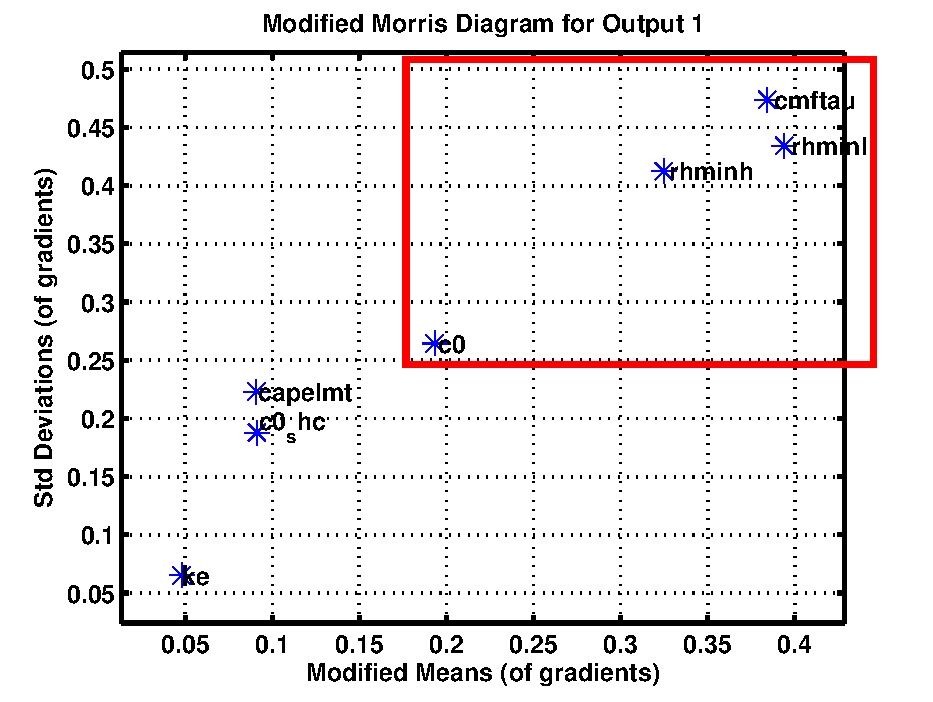
\includegraphics[width=8.3cm]{Morris}
\caption{Morris results}
\end{figure}

\begin{figure}[t]
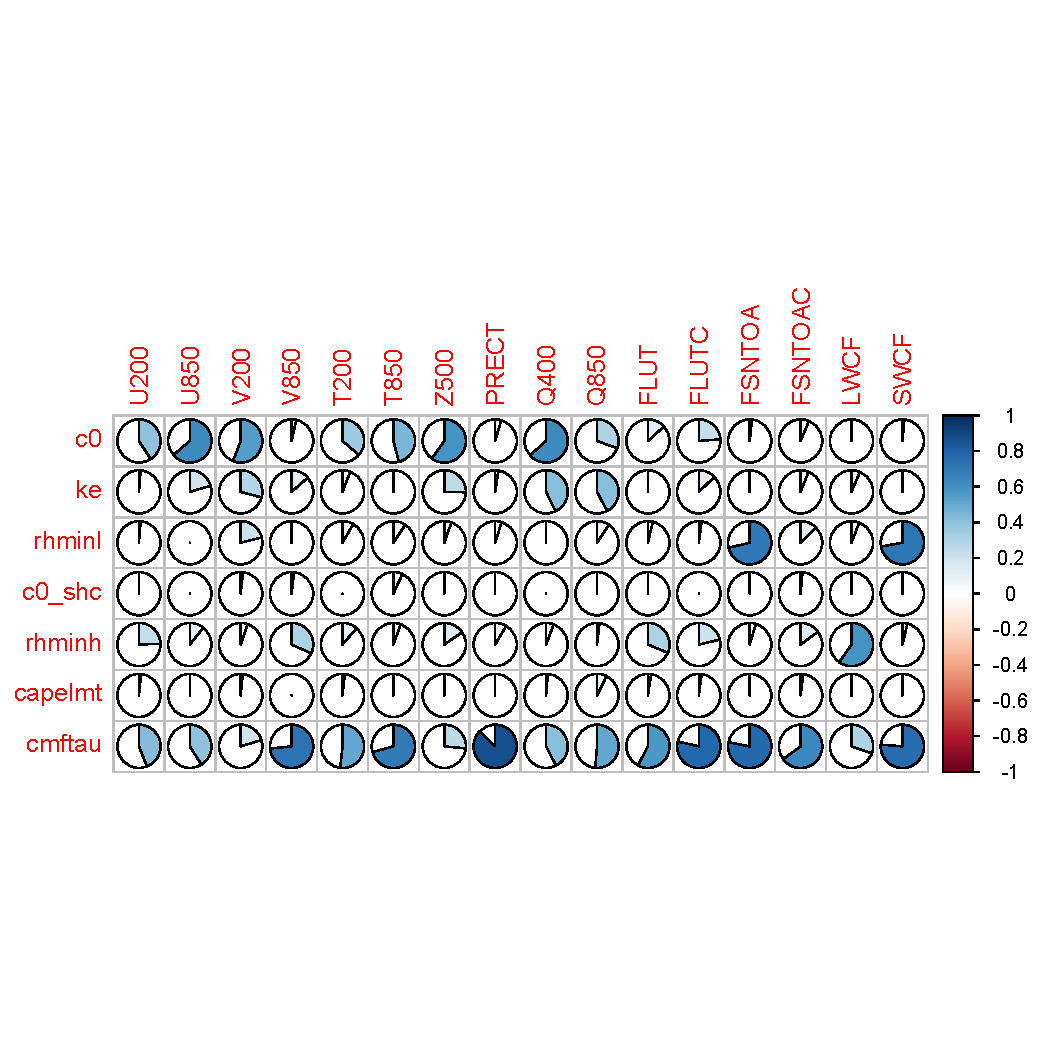
\includegraphics[width=8.3cm]{Sobol}
\caption{Sobol results}
\end{figure}

\begin{figure}[t]
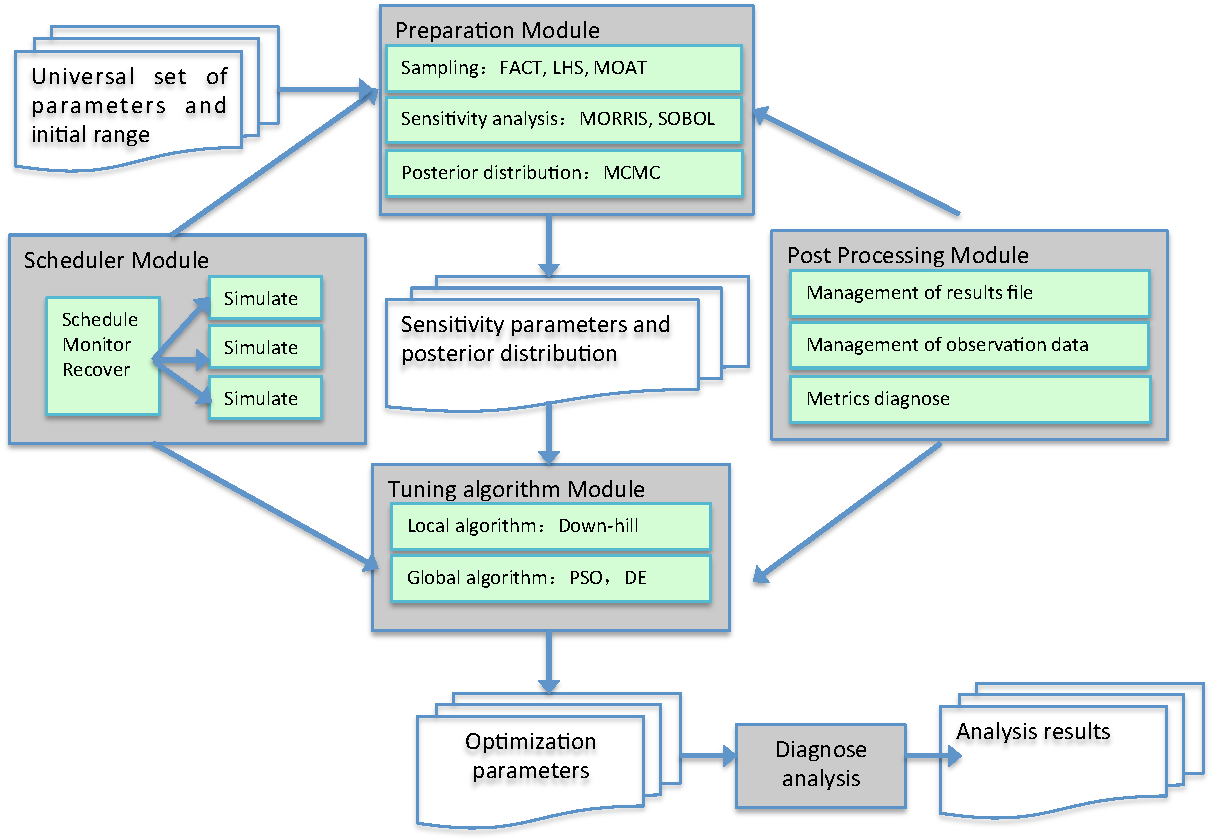
\includegraphics[width=15.3cm]{workflow}
\caption{calibration workflow}
\end{figure}

\begin{figure}[t]
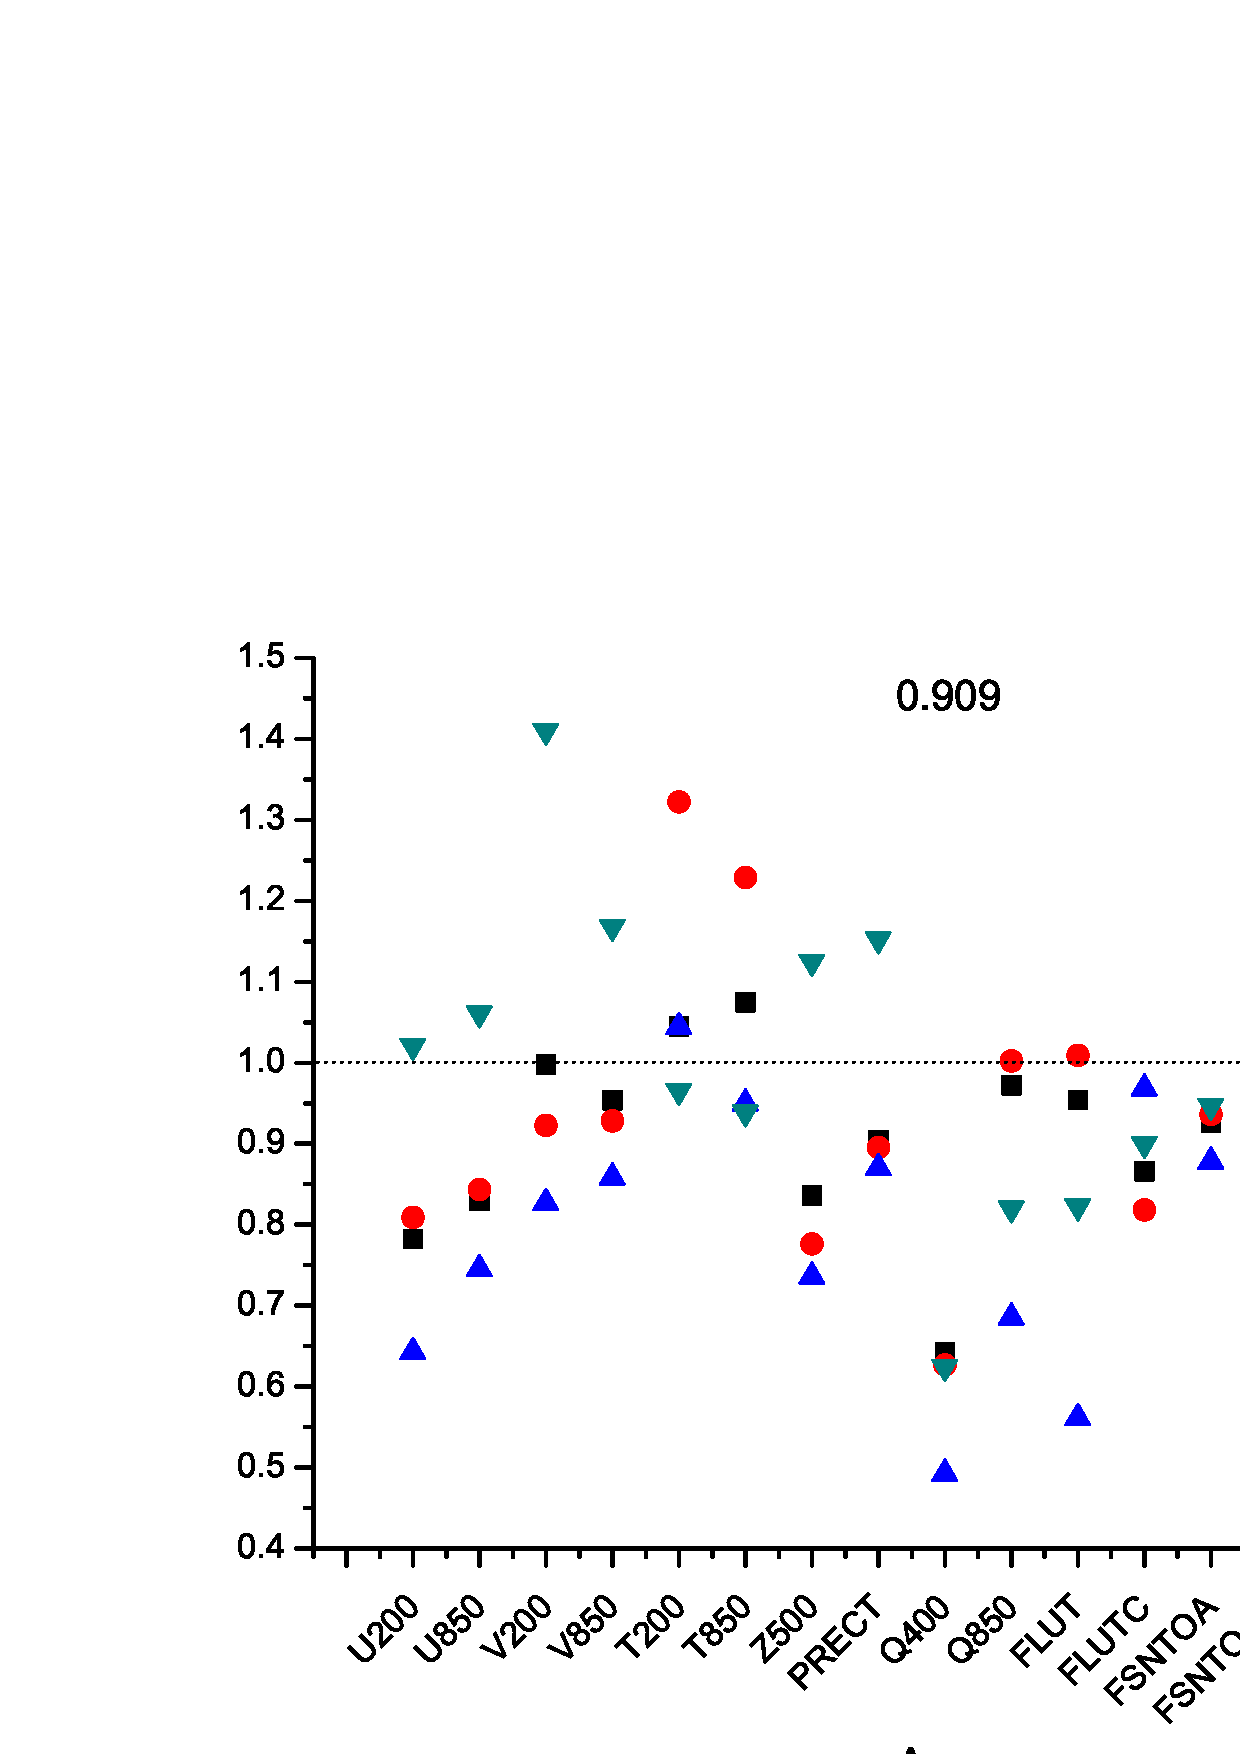
\includegraphics[width=15.3cm]{reg}
\caption{Metrics of each variables with the global, tropic, and northern / southern middle and high latitudes}
\end{figure}

\begin{figure}[t]
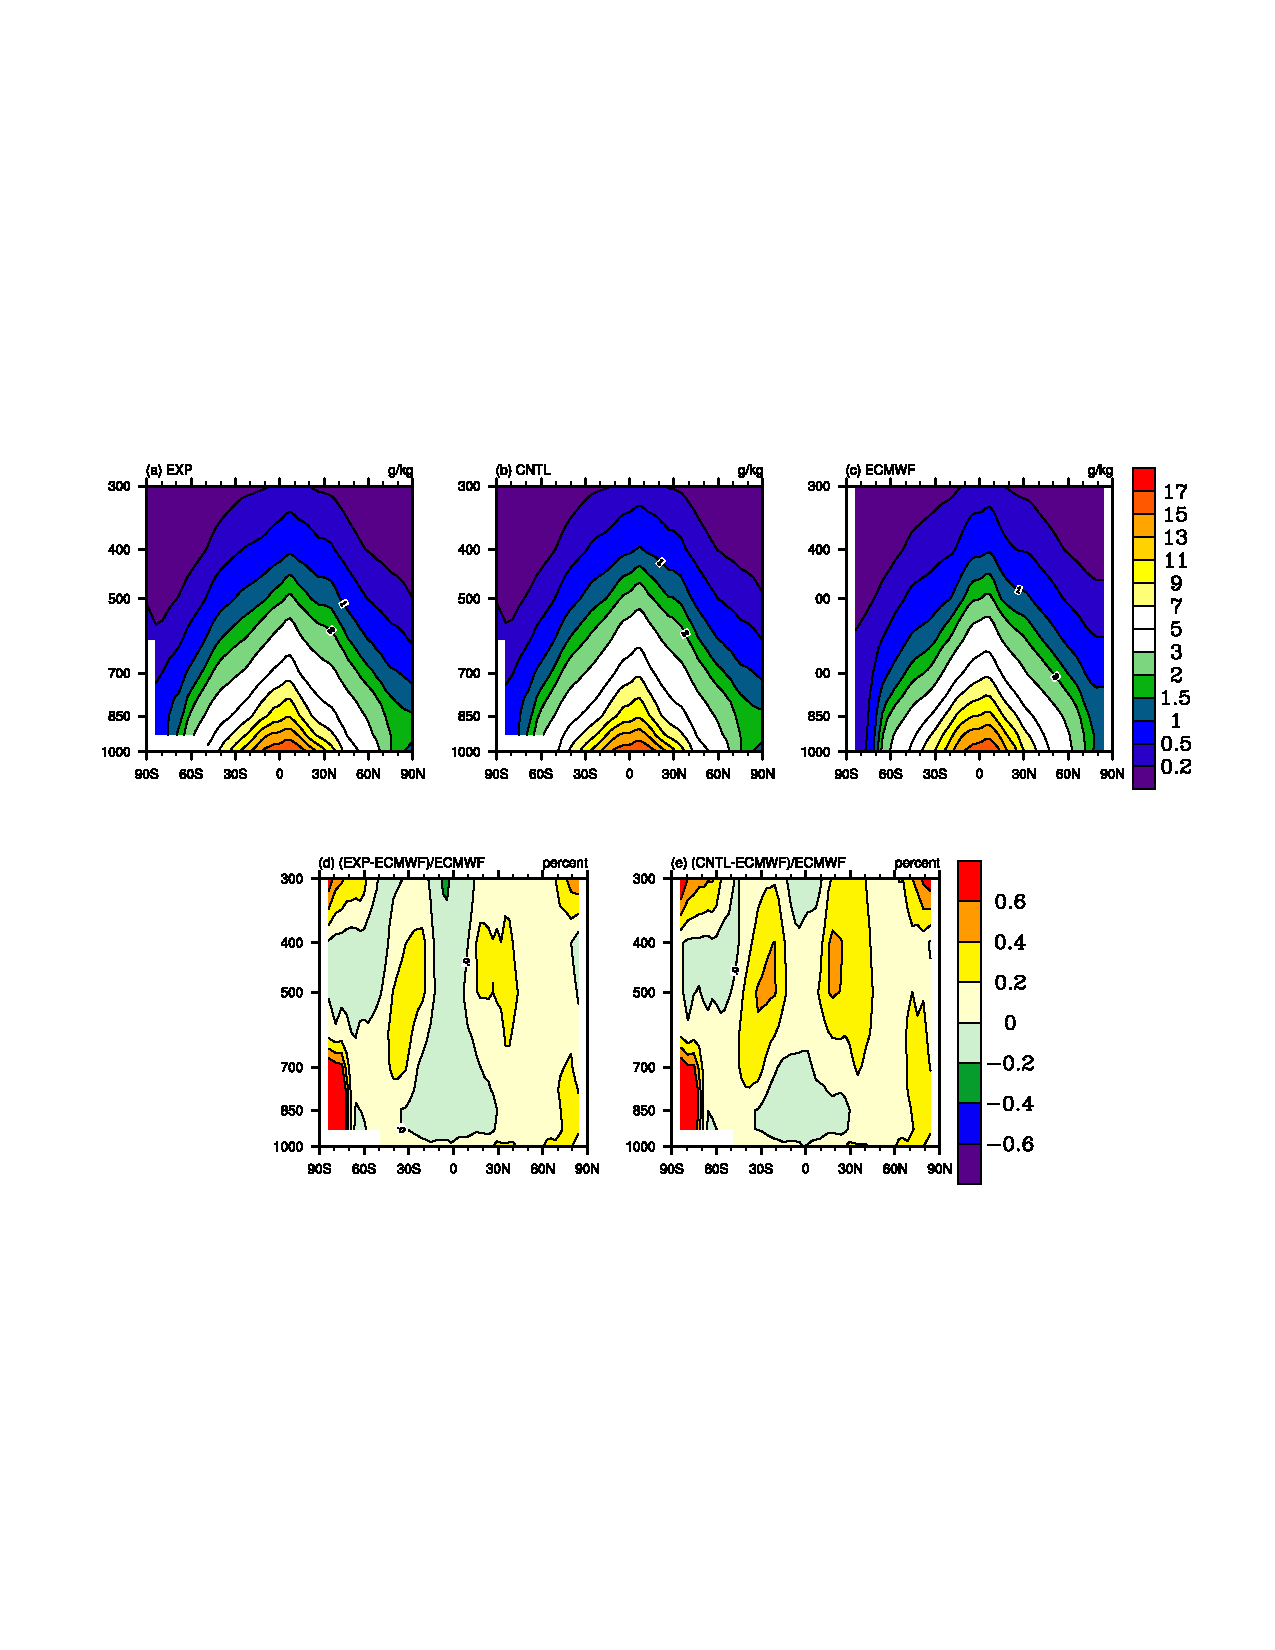
\includegraphics[width=15.3cm]{shum}
\caption{Pressure-latitude distributions of specific humidity of EXP (a), CNTL (b), observation (c), EXP-observation (d), and CNTL-observation (e).}
\end{figure}

\begin{figure}[t]
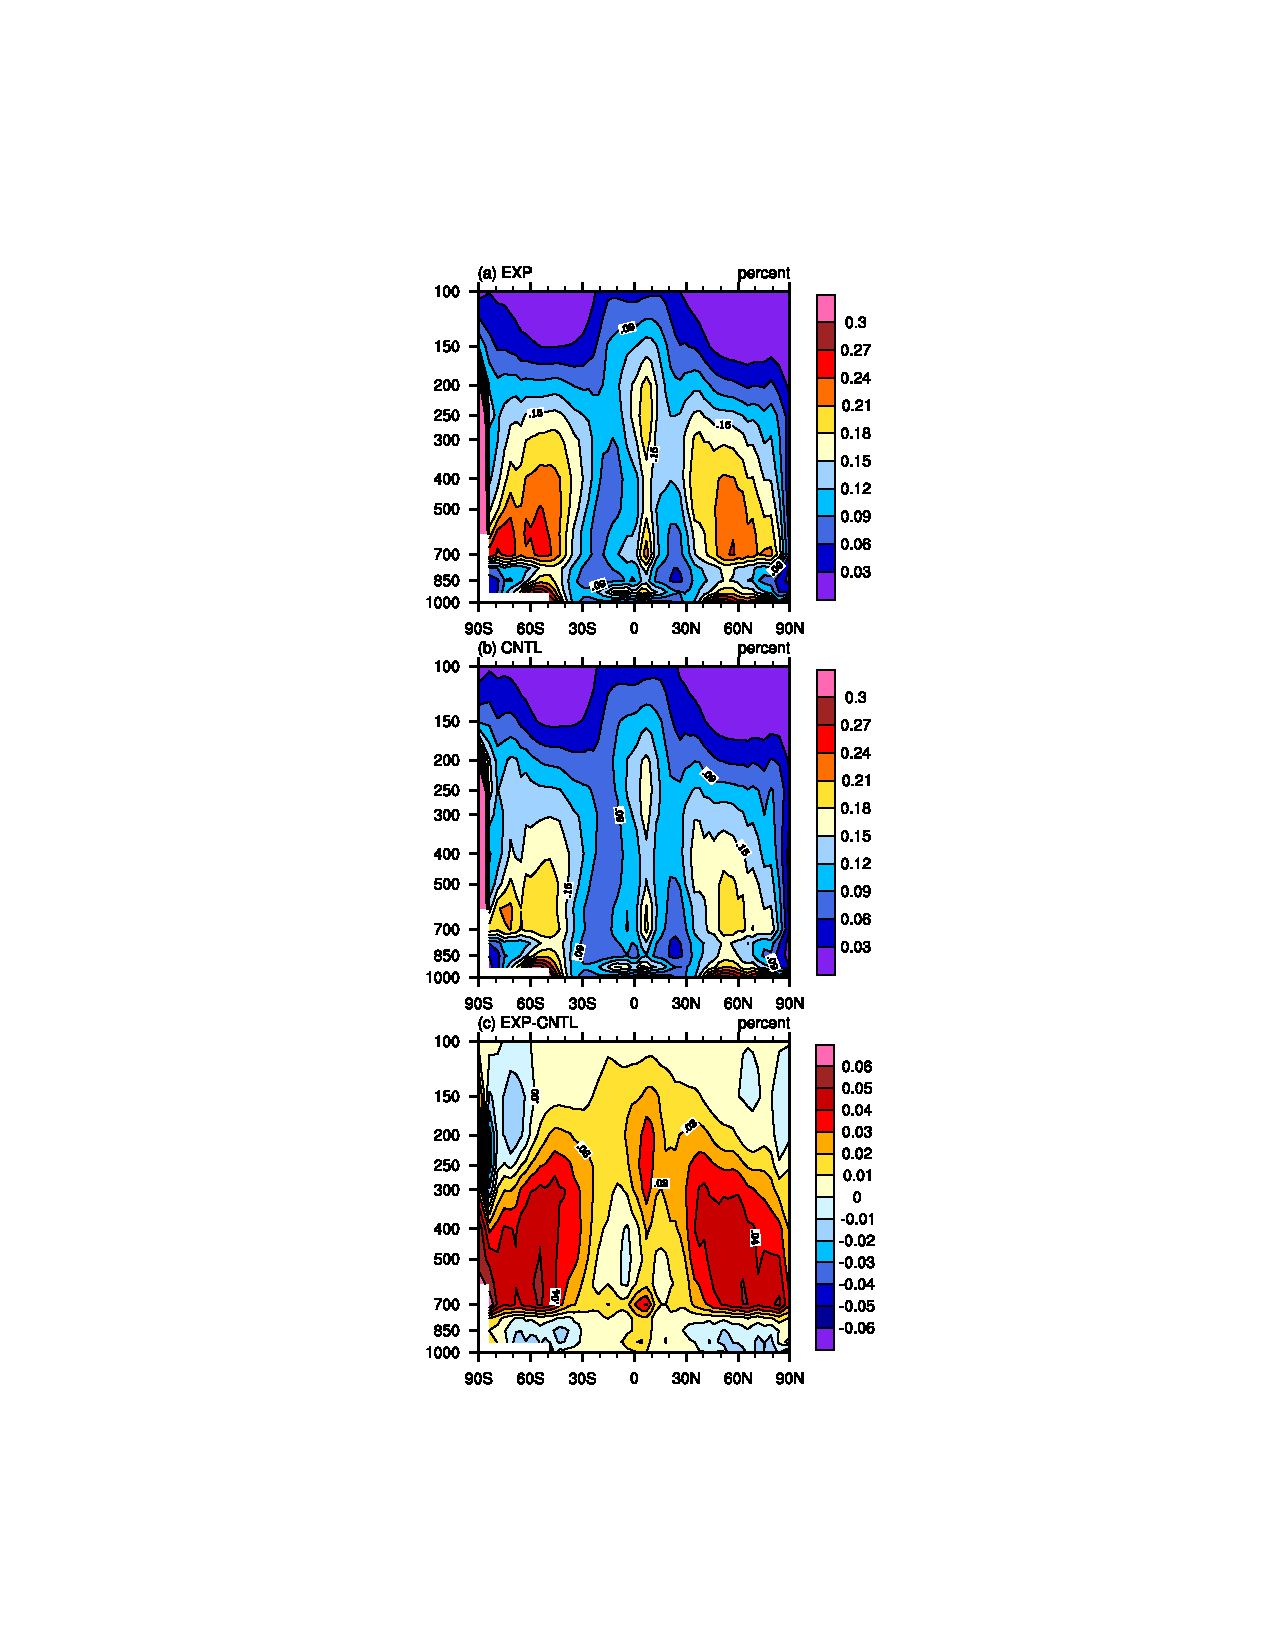
\includegraphics[width=15.3cm]{cloud}
\caption{Pressure-latitude distributions of cloud fraction of EXP (a), CNTL (b), and EXP-CNTL (c).}
\end{figure}

\begin{figure}[t]
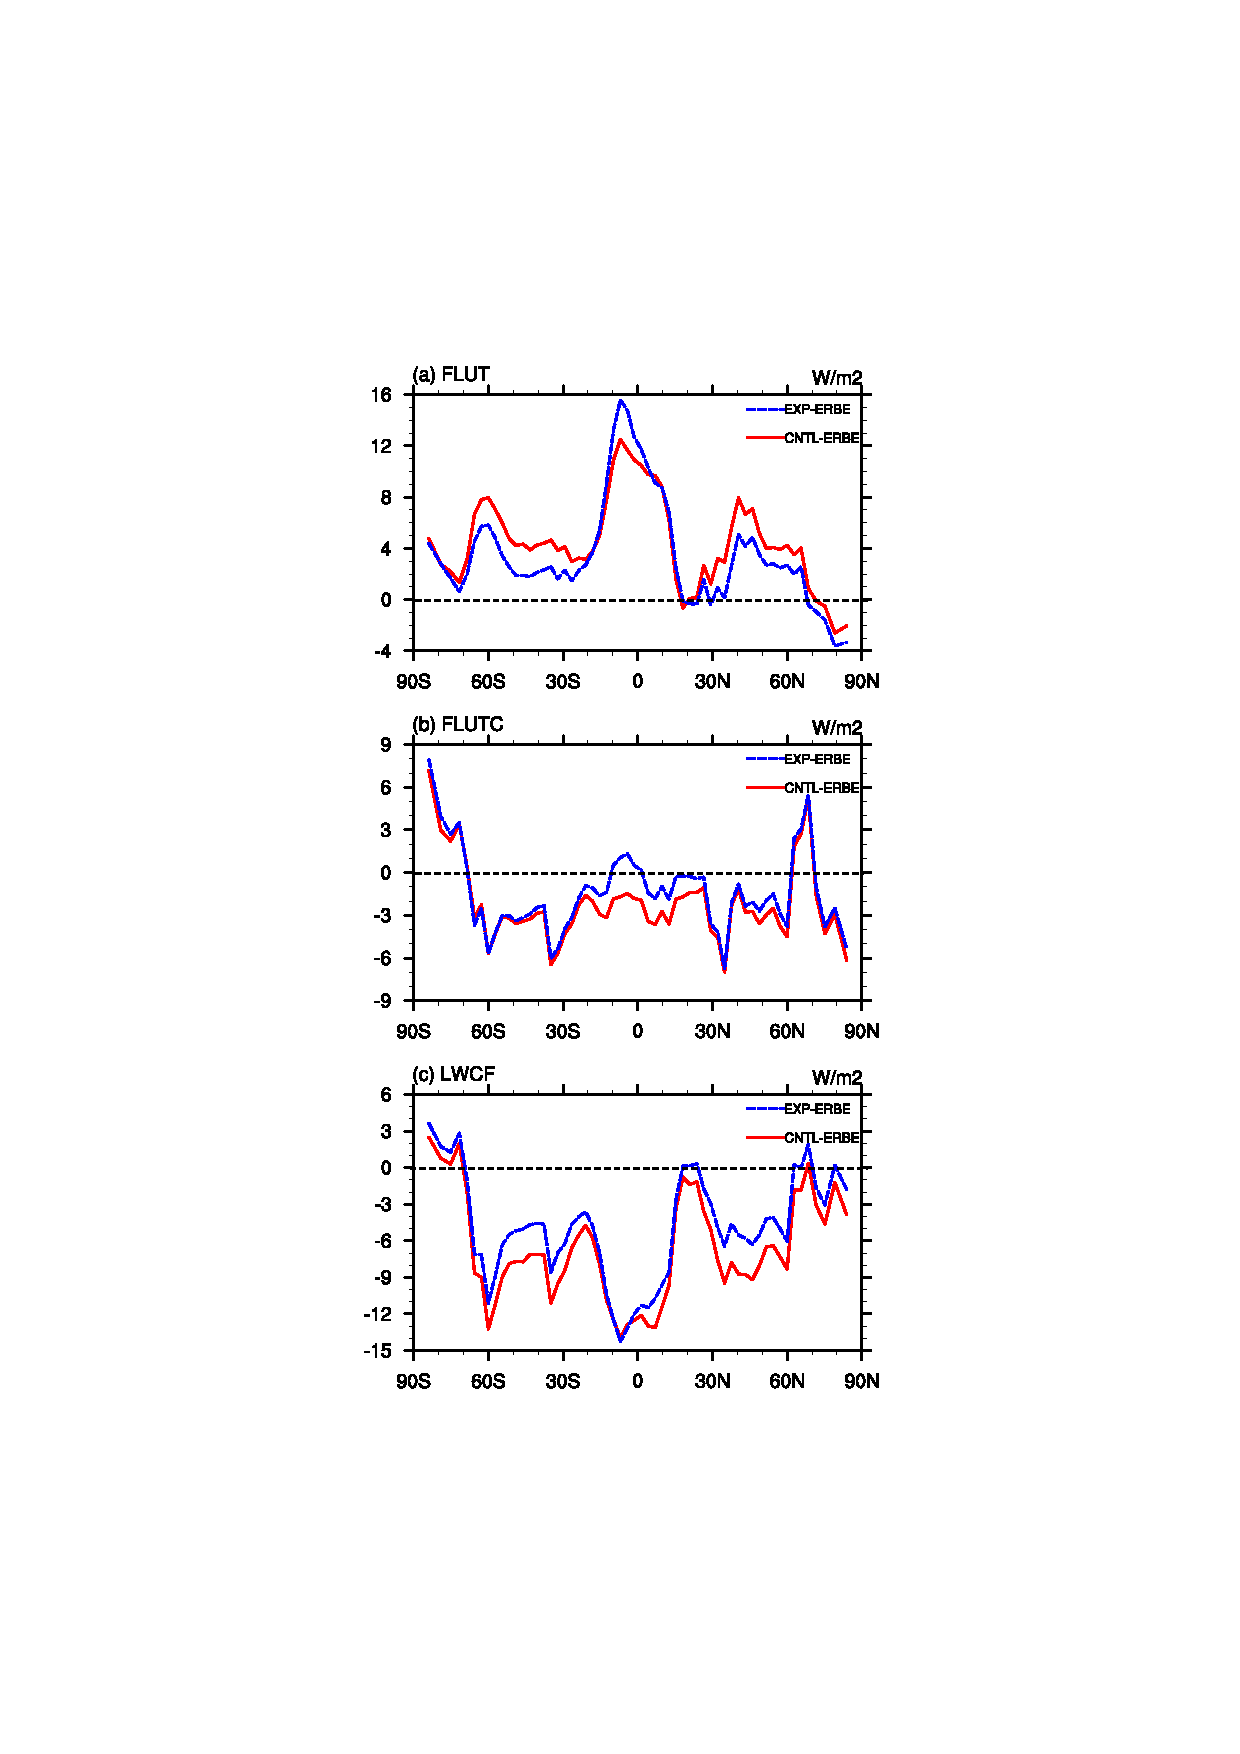
\includegraphics[width=12cm]{radiation_curve}
\caption{Meridional distributions of annual mean difference between EXP / CNTL and observation of FLUT (a), FLUTC (b), and LWCF (c).}
\end{figure}

\clearpage
%% TWO-COLUMN FIGURES

%f
%\begin{figure*}[t]
%\includegraphics[width=12cm]{FILE NAME}
%\caption{TEXT}
%\end{figure*}


%% TABLES
%%
%% The different columns must be seperated with a & command and should
%% end with \\ to identify the column brake.

%% ONE-COLUMN TABLE

%t

\begin{table}[t]
\caption{Initial selected uncertain parameters in GAMIL2}
\begin{tabular}{l l l c}
\tophline
Parameter & Description & Default & Range \\
\middlehline
c0 & rain water autoconversion coefficient for deep convection & 3.0e-4 & 1.e-4 $\sim$ 5.4e-3 \\
ke & evaporation efficiency for deep convection & 7.5e-6 & 5e-7 $\sim$ 5e-5 \\
capelmt & threshold value for cape for deep convection & 80 & 20 $\sim$ 200 \\
rhminl & threshold RH for low clouds & 0.915 & 0.8 $\sim$ 0.95 \\
rhminh & threshold RH for high clouds & 0.78 & 0.6 $\sim$ 0.9 \\
c0\_shc & rain water autoconversion coefficient for shallow convection & 5e-5 & 3e-5 $\sim$ 2e-4 \\
cmftau & characteristic adjustment time scale of shallow cape & 7200 & 900 $\sim$ 14400 \\
\bottomhline
\end{tabular}
\belowtable{} % Table Footnotes
\end{table}

\begin{table}[t]
\caption{Model output variables in the metrics}
\begin{tabular}{l l l l}
\tophline
Variable & Observation & Variable & Observation \\
\middlehline
Meridional wind at 850hPa   & ECMWF & Geopotential Z at 500hPa              & ECMWF \\
Meridional wind at 200hPa   & ECMWF & Total precipitation rate              & GPCP \\
Zonal wind at 850hPa        & ECMWF & Longwave cloud forcing                & ERBE \\
Zonal wind at 200hPa        & ECMWF & Shortwave cloud forcing               & ERBE \\
Temperature at 850hPa       & ECMWF & Long wave upward flux at TOA          & ERBE \\
Temperature at 200hPa       & ECMWF & Clearsky long wave upward flux at TOA & ERBE \\
Specific Humidity at 850hPa & ECMWF & Short wave net flux at TOA            & ERBE \\
Specific Humidity at 400hPa & ECMWF & Clearsky short wave net flux at TOA   & ERBE \\
\bottomhline
\end{tabular}
\belowtable{} % Table Footnotes
\end{table}

\begin{table}[t]
\caption{Fall factor samplings of parameters and metrics}
\begin{tabular}{l l l l l l l l l l l l}
\tophline
ID & c0 & rhminl & rhminh & cmftau & metrics & ID & c0 & rhminl & rhminh & cmftau & metrics \\
\middlehline
1  & 1.00E-04 & 0.915 & 0.78 & 7200 & 1.152 & 14 & 3.00E-04  & 0.875 & 0.78  & 7200  & 1.019     \\
2  & 3.00E-04 & 0.915 & 0.78 & 7200 & 1     & 15 & 3.00E-04  & 0.913 & 0.78  & 7200  & 1.007     \\
3  & 3.04E-04 & 0.915 & 0.78 & 7200 & 1.054 & 16 & 3.00E-04  & 0.95  & 0.78  & 7200  & 1.094     \\
4  & 5.08E-04 & 0.915 & 0.78 & 7200 & 1.017 & 17 & 3.00E-04  & 0.915 & 0.6   & 7200  & 1.00547   \\
5  & 7.13E-04 & 0.915 & 0.78 & 7200 & 0.987 & 18 & 3.00E-04  & 0.915 & 0.675 & 7200  & 1.027676  \\
6  & 9.17E-04 & 0.915 & 0.78 & 7200 & 1.01  & 19 & 3.00E-04  & 0.915 & 0.75  & 7200  & 1.023358  \\
7  & 1.12E-03 & 0.915 & 0.78 & 7200 & 1.04  & 20 & 3.00E-04  & 0.915 & 0.825 & 7200  & 1.028264  \\
8  & 1.33E-03 & 0.915 & 0.78 & 7200 & 1.044 & 21 & 3.00E-04  & 0.915 & 0.9   & 7200  & 1.160479  \\
9  & 2.55E-03 & 0.915 & 0.78 & 7200 & 1.075 & 22 & 3.00E-04  & 0.915 & 0.78  & 900   & 1.22922   \\
10 & 3.78E-03 & 0.915 & 0.78 & 7200 & 1.084 & 23 & 3.00E-04  & 0.915 & 0.78  & 4275  & 1.064064  \\
11 & 5.00E-03 & 0.915 & 0.78 & 7200 & 1.09  & 24 & 3.00E-04  & 0.915 & 0.78  & 7650  & 1.004806  \\
12 & 3.00E-04 & 0.8   & 0.78 & 7200 & 1.223 & 25 & 3.00E-04  & 0.915 & 0.78  & 11025 & 1.077167  \\
13 & 3.00E-04 & 0.838 & 0.78 & 7200 & 1.054 & 26 & 3.00E-04  & 0.915 & 0.78  & 14400 & 1.148265  \\
\bottomhline
\end{tabular}
\belowtable{} % Table Footnotes
\end{table}

\begin{table}[t]
\caption{Comparison with effective and efficiency}
\begin{tabular}{l l l l l}
\tophline
  & Optimal solution & $N_{step}$ & $N_{size}$ & Core hours \\
\middlehline
Down-hill simplex & 0.9585    & 80         & 1  & 14400 \\
PSO               & 0.911537  & 24         & 12 & 51840 \\
DE                & 0.942148  & 33         & 12 & 71280 \\
Dowmhill\_2\_steps  & 0.9256899 & 25+34    &  1 & 10620 \\
Downhill\_3\_steps  & 0.9098545 & 80+25+50 &  1 & 27900 \\
\bottomhline
\end{tabular}
\belowtable{} % Table Footnotes
\end{table}

\clearpage
%% TWO-COLUMN TABLE

%t
%\begin{table*}[t]
%\caption{TEXT}
%\begin{tabular}{column = lcr}
%\tophline

%\middlehline

%\bottomhline
%\end{tabular}
%\belowtable{} % Table Footnotes
%\end{table*}


%% NUMBERING OF FIGURES AND TABLES
%%
%% If figures and tables must be numbered 1a, 1b, etc. the following command
%% should be inserted before the begin{} command.

%\addtocounter{figure}{-1}\renewcommand{\thefigure}{\arabic{figure}a}


%% MATHEMATICAL EXPRESSIONS

%% All papers typeset by Copernicus Publications follow the math typesetting regulations
%% given by the IUPAC Green Book (IUPAC: Quantities, Units and Symbols in Physical Chemistry,
%% 2nd Edn., Blackwell Science, available at: http://old.iupac.org/publications/books/gbook/green_book_2ed.pdf, 1993).
%%
%% Physical quantities/variables are typeset in italic font (t for time, T for Temperature)
%% Indices which are not defined are typeset in italic font (x, y, z, a, b, c)
%% Items/objects which are defined are typeset in roman font (Car A, Car B)
%% Descriptions/specifications which are defined by itself are typeset in roman font (abs, rel, ref, tot, net, ice)
%% Abbreviations from 2 letters are typeset in roman font (RH, LAI)
%% Vectors are identified in bold italic font using \vec{x}
%% Matrices are identified in bold roman font
%% Multiplication signs are typeset using the LaTeX commands \times (for vector products, grids, and exponential notations) or \cdot
%% The character * should not be applied as mutliplication sign


%% EQUATIONS

%% Single-row equation

%\begin{equation}

%\end{equation}

%% Multiline equation



%\begin{align}
%& y=2+4x_1+4x_2-x_1^2-x_2^2+2sin(2x_1)sin(2x_2) \\
%& 0.5 \leq x_1, x_2 \leq 3.5
%\end{align}


%% MATRICES

%\begin{matrix}
%x & y & z\\
%x & y & z\\
%x & y & z\\
%\end{matrix}


%% ALGORITHM

\begin{algorithm}[htb]
\caption{Preprocessing the initial values of Downhill Simplex Algorithm} 
\label{alg:sequential-operation}
\begin{algorithmic}
%\STATE !********************************************
%\STATE !(1) Setting the initial values
%\STATE !******************************************** 
\STATE sampling\_sets=full\_factor\_sampling(parameters\_range)
\FOR{each initial $V_i$ of N+1 vertexes}
\STATE candidate\_init\_sets += min(i, sampling\_sets)
\ENDFOR
\WHILE{one parameter have the same values in the N+1 sets}
\STATE j=1
\STATE remove\_parameter\_set(the parameter set with higher metrics, candidate\_init\_sets)
\STATE candidate\_init\_sets += min(N+1+j, sampling\_sets)
\STATE j+=1
\ENDWHILE
\end{algorithmic}
\end{algorithm}

% \begin{algorithm}[htb]
% \caption{Downhill Simplex Algorithm} 
% \label{alg:sequential-operation}
% \begin{algorithmic}
% %\STATE !*********************************************
% %\STATE !(2) Downhill Simplex Algorithm
% %\STATE !*********************************************
% \WHILE {step=1,2..., until convergence}
% \STATE $V_h=$vertex with the highest metrics value
% \STATE $V_{l0}=$vertex with the lowest metrics value
% \STATE $V_{l1}=$vertex with the second lowest metrics value
% \STATE !***computing the center of gravity $V_g$ except for $V_h$***
% \STATE $V_g=\frac{1}{n}(\sum_{i=1}^{N+1} V_i - V_h)$ 
% \STATE !***computing the reflection vertex $V_r$ of $V_h$ based on $V_g$***
% \ENDWHILE
% \end{algorithmic}
% \end{algorithm}


%% CHEMICAL FORMULAS AND REACTIONS

%% For formulas embedded in the text, please use \chem{}

%% The reaction environment creates labels including the letter R, i.e. (R1), (R2), etc.

%\begin{reaction}
%% \rightarrow should be used for normal (one-way) chemical reactions
%% \rightleftharpoons should be used for equilibria
%% \leftrightarrow should be used for resonance structures
%\end{reaction}


%% PHYSICAL UNITS
%%
%% Please use \unit{} and apply the exponential notation

\end{document}
